\documentclass[10pt,a4paper]{article}
\usepackage[utf8]{inputenc}
\usepackage[T1]{fontenc}
\usepackage{amsmath}
\usepackage{amsthm}
\usepackage{amssymb}
\usepackage{graphicx}
\usepackage{mathtools}
\usepackage[ruled,vlined,linesnumbered]{algorithm2e}
\usepackage[left=2.50cm, right=2.50cm, top=2.0cm, bottom=2.0cm]{geometry}


\makeatother
\DeclareMathOperator*{\argmin}{argmin}
\DeclareMathOperator*{\Max}{\text{max}}
\DeclareMathOperator*{\E}{\mathbb{E}}
\newcommand{\Ei}[1]{\mathbb{E}_{#1}}
\DeclareMathOperator*{\Eik}{\mathbb{E}_{\mathit{i_k}}}
\DeclareMathOperator*{\Eikplus}{\mathbb{E}_{\mathit{i_{k+1}}}}
\newcommand{\Eiplus}[1]{\mathbb{E}_{i_{#1}}}
\DeclareMathOperator*{\LC}{\text{\textup{LC}}^1}
\DeclareMathOperator*{\grad}{\mathit{\nabla \!f}}
\DeclareMathOperator*{\argmax}{arg\;max}
\DeclareMathOperator*{\gradik}{\mathit{\nabla\!\fik}}
\DeclareMathOperator*{\Lmax}{\mathit{L_{max}}}
\newcommand{\R}{\mathbb{R}}
\newcommand{\st}{\text{s.t.} \;\;\;}
\newcommand{\Rn}{\mathbb{R}^n}
\newcommand{\ikplus}{i_{k+1}}
\newcommand{\wrefi}[2]{w_{r(#1, i_{#2})}}
\newcommand{\wref}[1]{\wrefi{#1}{#1}}
\newcommand{\fik}{f_{i_k}}
\newcommand{\fikofwstar}{\fik(w^*)}
\newcommand{\fofwstar}{f(w^*)}
\newcommand{\fii}[1]{f_{i_{#1}}}
\newcommand{\fikplus}{f_{i_{k+1}}}
\newcommand{\fiplus}[1]{f_{i_{#1}}}
\newcommand{\fimax}{f_i^{\text{max}}}
\newcommand{\fikmax}{\fik^{\text{max}}}
\newcommand{\bmax}{b_{\text{max}}}
\newcommand{\fmax}{f^{\text{max}}}
\newcommand{\fmaxk}[1]{f_{i_{#1}}^{\text{max}}}
\newcommand{\Lik}{L_{i_k}}
\newcommand{\Cik}{C_{i_k}}
\newcommand{\deltak}{\delta^{l_k}}
\newcommand{\deltakplus}{\delta^{l_k+1}}
\newcommand{\deltakminus}{\delta^{l_k-1}}
\newcommand{\etatilde}{\tilde{\eta}_{k,0}}
\newcommand{\muik}{\mu_{i_k}}
\newcommand{\etamax}{\eta^{\text{max}}}
\newcommand{\etamaxx}{\bar{\eta}^{\text{max}}}
\newcommand{\etamin}{\eta^{\text{min}}}
\newcommand{\etaminn}{\bar{\eta}^{\text{min}}}
\newcommand{\minimum}[2]{\min \left\{ #1, #2 \right \} }
\newcommand{\maximum}[2]{\max \left\{ #1, #2 \right \} }
\newcommand{\W}[1]{{\scriptscriptstyle W #1}}
\newcommand{\gradi}[1]{\nabla f_{i_{#1}} (w_{i_{#1}}) }
\makeatletter

\newtheorem{assumption}{Assumption}
\newtheorem{lemma}{Lemma}
\newtheorem{proposition}{Proposition}
\newtheorem{theorem}{Theorem}
\newtheorem{corollary}{Corollary}
\newtheorem{remark}{Remark}


\newcommand{\imgS}{.26}
\newcommand{\dir}{exp1/}
\newcommand{\model}{mlp}
\newcommand{\modelname}{mlp}


\newcommand{\mlp}{{\texttt{mnist|mlp}}}
\newcommand{\res}{{\texttt{cifar10|resnet34}}}
\newcommand{\dense}{{\texttt{cifar10|densenet121}}}
\newcommand{\ress}{{\texttt{cifar100|resnet34}}}
\newcommand{\denses}{{\texttt{cifar100|densenet121}}}
\newcommand{\fashion}{{\texttt{fashion|effb1}}}
\newcommand{\svhn}{{\texttt{svhn|wrn}}}
\newcommand{\wiki}{{\texttt{wiki2|encoder}}}
\newcommand{\ptb}{{\texttt{ptb|xl}}}
\newcommand{\mushrooms}{{\texttt{mushrooms}}}
\newcommand{\rcvone}{{\texttt{rcv1}}}
\newcommand{\ijcnn}{{\texttt{ijcnn}}}
\newcommand{\weighta}{{\texttt{w8a}}}

\title{Optimization Methods}
\author{Chapter 2: First Order Methods for Unconstrained Optimization}
\date{}
\begin{document}
	\maketitle
	\section{Descent Direction Methods}
	\noindent In this chapter we consider the unconstrained minimization problem
	\begin{equation*}
		\min_{x\in\Rn} \;\; f(x).
	\end{equation*}
The iterative algorithms that we will consider in this chapter take the form
\begin{equation*}
	x_{k+1} = x_k +t_k d_k \quad k=0,1, \dots,
\end{equation*}
where $d_k$ is the so-called direction and $t_k$ is the step size. We will limit ourselves to descent
directions, whose definition is now given.
\begin{definition}
	Let $f:\Rn\to\R$ with $f\in\C(\Rn)$ and $x\in \Rn$. A vector $0\neq d\in \Rn$ is called a descent direction of $f$ at $x$ if the directional derivative $f'(x,d)$ is negative, i.e., 
	\begin{equation*}
		f'(x,d)= \grad(x)^T d < 0.
	\end{equation*}
\end{definition}
\noindent In particular, by taking small enough steps, descent directions lead to a decrease of the objective function.
\begin{lemma}[descent property of descent directions]
	Let $f:\Rn\to\R$ with $f\in\C(\Rn)$ and let $x\in \Rn$. Suppose that $d$ is a descent direction of $f$ at $x$. Then, there exists $\epsilon>0$ such that 
	\begin{equation*}
		f(x+td) < f(x) \quad \forall \, t \in (0,\epsilon].
	\end{equation*} 
\end{lemma}
\begin{proof}
	Since $f'(x,d)<0$, it follows from the definition of the directional derivative that 
	\begin{equation*}
		\lim_{t\to 0^+}\frac{f(x+td)-f(x)}{t} = f'(x,d) <0.
	\end{equation*}
Therefore, there exists an $\epsilon>0$ such that 
\begin{equation*}
	\frac{f(x+td)-f(x)}{t}<0,
\end{equation*}
for any $t\in(0,\epsilon)$
\end{proof}
\begin{algorithm}[H]\label{alg}
	\caption{Schematic Descent Directions Method}
	
	\KwIn{$x_0\in \Rn$}
	
	$k = 0$
	
	\While{Termination criterion is not satisfied}{
				
			Pick a descent direction $d_k$
			
			Find a step size $t_k$ satisfying $f(x_k+t_kd_k)<f(x_k)$
			
			$x_{k+1} = x_k+t_kd_k$
			
			$k = k+1$
		}
\end{algorithm}
\noindent Various choices are still unspecified: which direction to take, how to select the step size, what termination criterion to use.
\section{Gradient Method}
\noindent The most important choice in the algorithm above concerns the selection of the descent direction. One obvious choice is to pick the steepest (normalized) direction, i.e., $d_k =-\grad(x_k)/||\grad(x_k)||$. In fact, this direction minimizes the directional derivatives between all normalized directions. 
\begin{lemma}
	Let $f:\Rn\to\R$ with $f\in\C(\Rn)$ and let $x\in\Rn$ be non-stationary (i.e., $\grad(x)\neq0$). Then the optimal solution of the problem
	\begin{equation*}
		\begin{split}
			\min \;\; &f'(x,d),\\
			\st& ||d||=1.
		\end{split}
	\end{equation*}
is $d=-\frac{\grad(x)}{||d||}$.
\end{lemma}
\begin{proof}
	As $f\in \C(\Rn)$ and by Cauchy-Schwarz, we have 
	\begin{equation*}
		f'(x,d)=\grad(x)^Td \geq -||\grad(x)||\cdot ||d|| = -||\grad(x)||.
	\end{equation*}
Thus, $-||\grad(x)||$ is a lower bound for the optimal value of the problem. On the other hand, by plugging  $d = -\grad(x)/||\grad(x)||$ in the objective function we get 
\begin{equation*}
	f'\left(x,-\frac{\grad(x)}{||\grad(x)||}\right)=-\grad(x)^T\left(\frac{\grad(x)}{||\grad(x)||}\right)= -||\grad(x)||,
\end{equation*}
and we thus come to the conclusion that the lower bound is attained at $d=-\frac{\grad(x)}{||d||}$.
\end{proof}
\noindent Thus, the gradient method selects $d_k = -\grad(x_k)$ which is obviously a descent direction, i.e., 
\begin{equation*}
\grad(x_k)^Td_k = -\grad(x_k)^T\grad(x_k) = -||\grad(x)||^2.
\end{equation*}
\noindent To define an implementable method, the second important choice we have to make is the selection of the step size $t$. In particular, this will be clearer once we provide the Descent Lemma below, which require the gradient to be Lipschitz continuous. 
\begin{definition}[Lipschitz Continuous Gradient]
	$\grad(x)$ is said to be Lipschitz continuous if 
	\begin{equation*}
		|| \grad(x) -\grad(y)|| \leq L ||x-y|| \quad \forall x,y \in \Rn.
	\end{equation*}
The class of functions with Lipschitz continuous gradient with constant $L$ is denoted by $\LC(\Rn)$.
\end{definition}
\begin{theorem}
	Let $f\in\Cii(\Rn)$. Then the following two claims are equivalent:
	\begin{itemize}
		\item[(a)] $f\in \LC(\Rn)$
		\item[(b)] $||\hess(x)||\leq L \quad \forall x\in \Rn$.
	\end{itemize}
\begin{proof}
	$(b)\Rightarrow (a)$. Suppose that $||\hess(x)||\leq L \quad \forall x\in \Rn$. By the fundamental theorem of calculus we have $\forall x,y \in \Rn$
	\begin{equation*}
		\begin{split}
			\grad(y)=\grad(x) + \int_{0}^{1} \hess(x+t(y-x)) (y-x) dt = \grad(x) + \left(\int_{0}^{1} \hess(x+t(y-x)) dt  \right) \cdot (y-x)
		\end{split}
	\end{equation*}
Thus, 
\begin{equation*}
	\begin{split}
		||\grad(y)-\grad(x)|| &= \left \| \left(\int_{0}^{1} \hess(x+t(y-x)) dt  \right) \cdot (y-x)\right \|\\
		&\leq \left\|\int_{0}^{1} \hess(x+t(y-x)) dt  \right\| \cdot \|(y-x) \|\\
		& \leq \left(\int_{0}^{1}|| \hess(x+t(y-x))|| dt  \right)\cdot \|(y-x) \|\\
		& \leq L \|(y-x) \|
	\end{split}
\end{equation*}
	$(a)\Rightarrow (b)$. Exercise.
\end{proof}
\end{theorem}
\begin{lemma}[Descent Lemma (part 1)] Let $f\in \LC(\Rn)$. Then for any $x,y \in \Rn$
	\begin{equation*}
		f(y) \leq f(x) + \grad(x)^T(y-x) + \frac{L}{2} \|x-y\|^2.
	\end{equation*}
\end{lemma}
\begin{proof}
From the fundamental theorem of calculus and differentiability of $f$ we have 
\begin{equation*}
	\begin{split}
		f (y) & = f(x) + \int_{0}^{1} \grad((1-t)x + t y)^T\! (y-x) \; dt\\
		& = f(x) + \int_{0}^{1} \grad((1-t)x + t y)^T\! (y-x) - \grad(x)^T(y-x) \; dt + \grad(x)^T(y-x)\\ 
		&\leq f(x) + \int_{0}^{1} \| \grad((1-t)x + t y) - \grad(x)\|\! \cdot\! \|y-x\| \; dt + \grad(x)^T(y-x)\\  
		& \leq f(x) + \int_{0}^{1} L \| t(y-x) \|\! \cdot\! \|y-x\| \; dt + \grad(x)^T(y-x)\\
		& = f(x) + L\|y-x\|^2 \cdot \frac{t^2}{2} \Big|_0^1 + \grad(x)^T(y-x)\\
		& = f(x) + \grad(x)^T(y-x) + \frac{L}{2} \|y-x\|^2,
	\end{split}
\end{equation*}
where the second inequality follows from the Lipschitz continuity of $\grad$.
\end{proof}
\begin{lemma}[Descent Lemma (part 2)]\label{lemma:descent} Let $f\in \LC(\Rn)$. Then for any $x \in \Rn$ and $t>0$
	\begin{equation*}
		f(x) - f(x-t\grad(x)) \geq t (1-\frac{Lt}{2}) \| \grad(x)\|^2.
	\end{equation*}
\end{lemma}
\begin{proof}
	The result simply follows by applying the descent lemma (prequel) on $x$ and $y=x-\grad(x)$
	\begin{equation*}
		f(x-t\grad(x))\leq f(x) -t ||\grad(x)\|^2 + \frac{Lt^2}{2} \|\grad(x)\|^2 = f(x) - t (1-\frac{Lt}{2}) \| \grad(x)\|^2
	\end{equation*}
\end{proof}
\noindent In particular, this holds for $x=x_k$ and $x_{k+1} = x_k -t\grad(x_k)$,
\begin{equation*}
	f(x_k) - f(x_{k+1}) \geq t (1-\frac{Lt}{2}) \| \grad(x_k)\|^2,
\end{equation*}
which in turns implies that if we select $t\in (0,\frac{2}{L})$ we ensure a decrease of the objective function at each iteration. In particular, if we want to achieve the largest guarantee bound on the decrease at each iteration $k$, then we seek the maximum of $t (1-\frac{Lt}{2})$ w.r.t. $t$, which is attained at the vertex of the parabola $t_v= \frac{-b}{2a}=\frac{1}{L}$ with a decrease that becomes
\begin{equation}\label{eq:decrease}
	f(x_k) - f(x_{k+1}) \geq \frac{1}{2L} \| \grad(x_k)\|^2.
\end{equation}
At this point we can write down the Gradient Method in terms of an implementable algorithm.

\begin{algorithm}[H]\label{gd}
	\caption{Gradient Descent (GD) Method}
	
	\KwIn{Pick $x_0\in \Rn$ arbitrarly, chose $\epsilon>0$ (e.g., $10^{-4}$).}
	
	$k = 0$
	
	\While{$\|\grad(x_k)\|> \epsilon$}{
		
		$x_{k+1} = x_k - \frac{1}{L} \grad(x_k)$
		
		$k = k+1$
	}
\end{algorithm}
\noindent Let us now prove convergence for GD, in particular that $\grad(x_k)$ goes to zero.
\begin{theorem}[Convergence of GD]\label{thm:GD_convergence}
	Let $f\in \LC(\Rn)$ and let $\{x_k\}_k$ be a sequence generated by Algorithm \ref{gd} for solving $\min_{x\in\Rn}\;f(x)$. Assume that $f$ is bounded from below over $\Rn$, i.e., there exists $m\in \R$ such that $f(x)>m \;\; \forall\, x\in \Rn$. Then we have the following
	\begin{itemize}
		\item[(a)] The sequence $\{f(x_k)\}_k$ is nonincreasing. In addition, for any $k\geq 0$, $f(x_{k+1}) < f(x_k)$ unless $\grad(x_k)=0$.
		\item[(b)] $\grad(x_k) \to 0$ as $k\to \infty$.
	\end{itemize}
\end{theorem}
\begin{proof}
	(a) directly follows from \eqref{eq:decrease}, as $f(x_{k+1}) < f(x_k)$ and the equality $f(x_{k+1}) = f(x_k)$ only holds when $\grad(x_k)=0$.
	(b) Since the sequence $\{f(x_k)\}_k$ is nonincreasing and bounded from below, it converges. Thus, $f(x_k) - f(x_{k+1}) \to 0$ as $k\to \infty$, which combined with \eqref{eq:decrease} implies that $\|\grad(x_k)\|\to 0$ as $k\to \infty$.  
\end{proof}
\noindent Moreover, we can provide the rate of convergence of GD.
\begin{theorem}[Rate of Convergence of GD]
	Under the setting of Theorem \ref{thm:GD_convergence}, let $f^*$ be the limit of the convergent sequence $\{f(x_k)\}_k$. Then for any $T=0,1, \dots$
	\begin{equation}\label{eq:convergence_rate}
		\min_{k=0,1,\dots, T} \| \grad(x_k) \|\leq \sqrt{\frac{2L (f(x_0) -f^*)}{T+1}}.
	\end{equation}
Moreover, Algorithm \ref{gd} has an iteration complexity of $\BigO(\epsilon^{-2})$.
\end{theorem}
\begin{proof}
	Summing the inequality \eqref{eq:decrease} over $k=0, 1, \dots, T$, we obtain 
	\begin{equation}\label{eq:tower}
		f(x_0) - f(x_{T+1}) \geq \frac{1}{2L}\sum_{k=0}^{T} \|\grad(x_k)\|^2
	\end{equation}
from which we get \eqref{eq:convergence_rate}, because the RHS can be lower bounded by $\frac{T+1}{2L} \min_{k=0,1,\dots, T} \| \grad(x_k)\|^2$.
If $\|\grad(x_k)||>\epsilon$ for the first $k_\epsilon$ iterations, from \eqref{eq:tower} used with $T=k_\epsilon-1$ we also get that 
\begin{equation*}
	f(x_0) -f^* \geq  f(x_0) - f(x_{k_\epsilon}) > \frac{k_\epsilon}{2L} \epsilon^2, 
\end{equation*}
thus $k_\epsilon< 2L(f(x_0) -f^*) \epsilon^{-2}$, which concludes the proof.
\end{proof}

\section{Line search methods}
The gradient method as defined above can only be employed when we know or we can compute the Lipschitz constant $L$, on the other hand, we would like to have a general method that can be applied on any unconstrained optimization problem. An alternative for selecting the step size is provided by line search methods. Consider a direction $d_k$, one option would be to exactly minimize along the direction $d_k$, i.e., \textbf{exact line search}
\begin{equation*}
	t_k \in \argmin_{t>0} f(x_k+t d_k).
\end{equation*}
However, this approach is not always viable and even when it is, it might be costly. Another option is instead that of accepting a step that will make the function value decrease "sufficiently", namely to apply an \textbf{inexact line search}. In particular, the first line search proposed in the literature is called Armijo line search \cite{armijo66a} and it requires the following
\begin{equation}\label{eq:armijo}
	f(x_k +t_k d_k) \leq f(x_k) + \alpha t_k\grad(x_k)^Td_k.
\end{equation}
Notice that if we define $\phi(t)=f(x_k+td_k)$ we can rewrite the inequality above as
\begin{equation*}
\phi(t_k) \leq \phi(0) + \alpha t_k \phi'(0) \qquad \with \alpha \in (0,1).
\end{equation*}
As depicted in Figure 1, the condition requires that the new function value $\phi(t_k)$ stays below the line passing for $(0,\phi(0))$ and with $\alpha\phi'(0)$ as inclination. Notice that as $\phi'(0)<0$ and $\alpha<1$, the line $y=\phi(0) +\alpha t_k \phi'(0)$ is not as inclined as the tangent in 0. The way for selecting a step $t_k$ that satisfies \eqref{eq:armijo} is suggested by the figure.
\begin{figure}
	\centering
	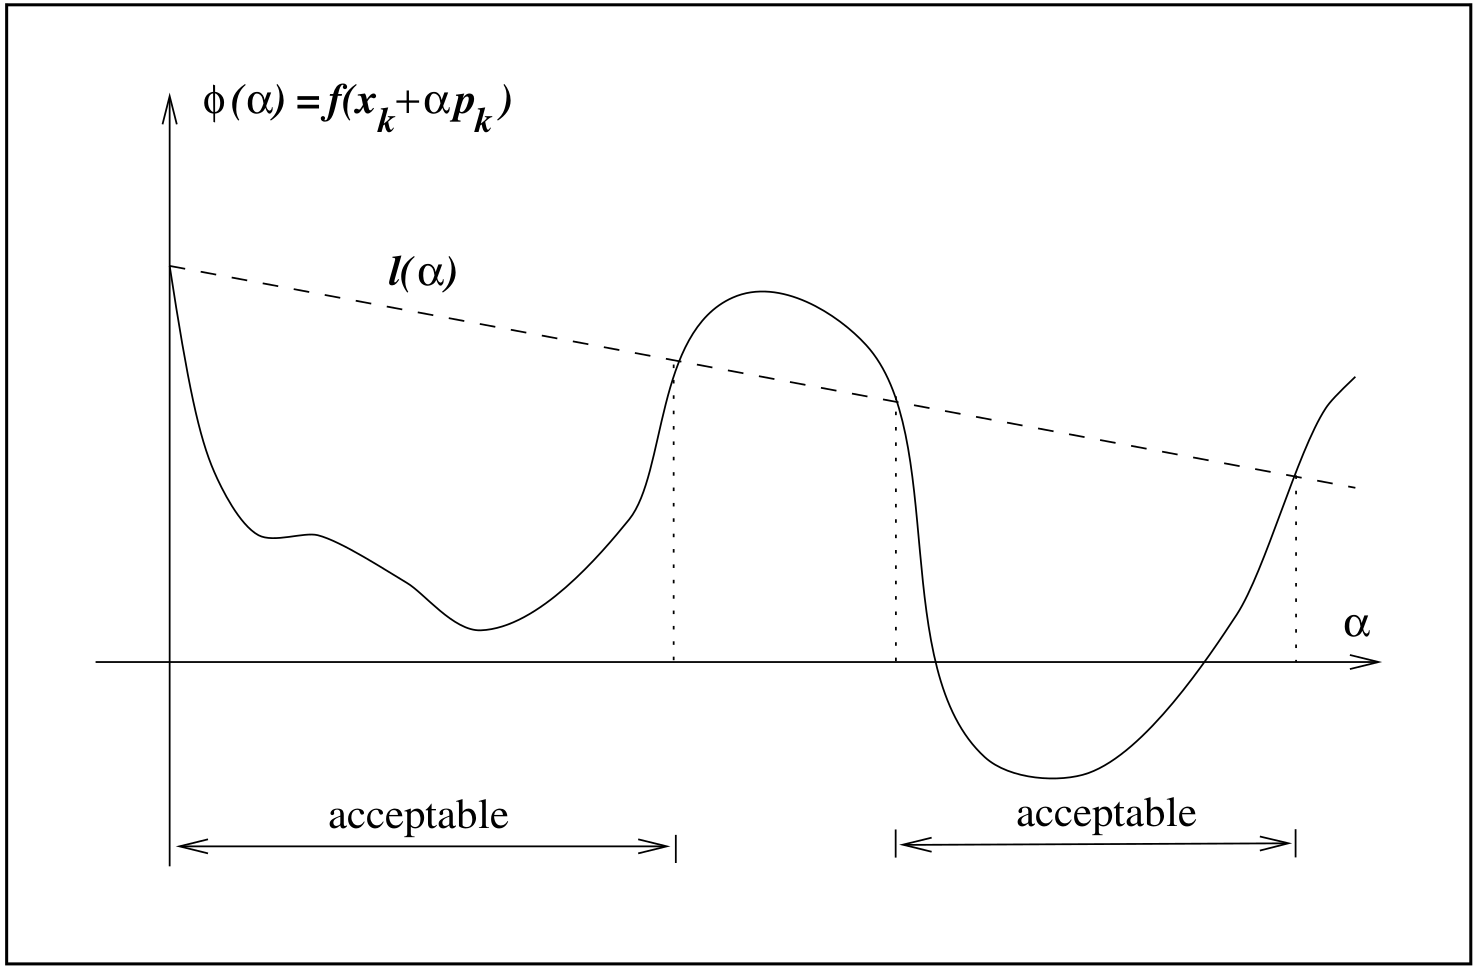
\includegraphics[width=0.5\linewidth]{lines}
	\caption{The figure represents the Armijo line search condition (the notation in this figure is different from the text, replace $\alpha$ in the figure with $t$ from the text.)}
\end{figure}
In particular, the method is called backtracking and it is described below.
\begin{algorithm}[H]\label{alg:armijo}
	\caption{Backtracking on Armijo line search}
	
	\KwIn{Pick $s>0$, $\alpha,\beta \in(0,1)$.}
	
	$i=0$	
	
	\Do{$f(x_k +t_k d_k) > f(x_k) + \alpha t_k \grad(x_k)^Td_k$}{
		
		$t_k = s \beta^i$
		
		$i=i+1$
	}
	
\end{algorithm}
\noindent Let us first show that this method terminates in a finite amount of steps
\begin{lemma} \label{lemma:finite_termination}
	Let $f\in \LC(\Rn)$, $x\in \Rn$ and $d\in \Rn$ be a descent direction. Then Algorithm \ref{alg:armijo} terminates in a finite amount of steps with a $t_k>0$ that satisfies \eqref{eq:armijo}. Moreover, one of the following holds
	\begin{itemize}
		\item[(a)] $t_k=s$
		\item[(b)] $t_k\leq \beta s$ such that $f(x_k +\frac{t_k}{\beta} d_k) > f(x_k) + \alpha \frac{t_k}{\beta} \grad(x_k)^Td_k$
	\end{itemize}
Consequently, with $d_k = -\grad(x_k)$ we get $t_k \geq \min \left\{s, \frac{2(1-\alpha)\beta}{L} \right \}$.
\end{lemma}
\begin{proof}
	Let us first prove that the algorithm terminates in a finite amount of steps. By contradiction there are no finite value of $i$ for which \eqref{eq:armijo} is satisfied, that is 
	\begin{equation*}
		\frac{f(x_k +s \beta^i d_k)- f(x_k)}{s \beta^i} > \alpha \grad(x_k)^Td_k.
	\end{equation*}
Given $\beta<1$ we have that $\lim_{i\to \infty} \beta^i =0$ and thus, with $i\to \infty$ the LHS of the inequality above is the directional derivative of $f$ along $d_k$. In particular, we get
\begin{equation*}
	\grad(x_k)^Td_k \geq \alpha\grad(x_k)^Td_k,
\end{equation*}
which is a contradiction, as $\grad(x_k)^Td_k<0$ and $\alpha <1$.
Following the steps of the algorithm, either the first guess $s$ is accepted or $t_k\leq s\beta$. In the second case, given $t_k$ the outcome of the algorithm, the step size before the last backtracking ($\frac{t_k}{\beta}$) was surely not accepted, from which (b) follows.
\par Now, we can replace $t=\frac{t_k}{\beta}$ in Lemma \ref{lemma:descent} with $x=x_k$ to get
\begin{equation*}
	f(x_k -\frac{t_k}{\beta} \grad(x_k)) \leq f(x_k) - \frac{t_k}{\beta} \left(1-\frac{L t_k}{2\beta}\right) \| \grad(x_k)\|^2
\end{equation*}
which combined with $(b)$ with $d_k=-\grad(x_k)$ implies
\begin{equation*}
	\frac{t_k}{\beta}\left(1-\frac{L t_k}{2\beta}\right) < \alpha\frac{t_k}{\beta}
\end{equation*}
and consequently $t_k>\frac{2(1-\alpha)\beta}{L}$, which together with $(a)$ concludes the proof.
\end{proof}
\noindent We can now provide a version of the GD method that is independent from $L$.\\
\begin{algorithm}[H]\label{alg:gd_armijo}
	\caption{Gradient Descent (GD) Method with Armijo Line Search}
	
	\KwIn{Pick $x_0\in \Rn$ arbitrarly, chose $\epsilon>0$ (e.g., $10^{-4}$).}
	
	$k = 0$
	
	\While{$\|\grad(x_k)\|> \epsilon$}{
		
		$t_k \leftarrow$ Armijo Line Search (Algorithm \ref{alg:armijo})
		
		$x_{k+1} = x_k - t_k \grad(x_k)$
		
		$k = k+1$
	}
\end{algorithm}
\noindent Notice that to prove convergence of Algorithm \ref{alg:gd_armijo} it suffices to show that also in this case we can derive a decrease as in \eqref{eq:decrease}. In particular, from the Lemma above, we get
\begin{equation*}
	f(x_k) - f(x_{k+1}) \geq \alpha  \min \left \{s, \frac{2(1-\alpha)\beta}{L} \right \} \| \grad(x_k)\|^2.
\end{equation*}
The iteration complexity of Algorithm \ref{alg:gd_armijo} is the same as that of GD (Algorithm \ref{gd}), however the cost of each iteration is different, as we have an internal procedure (Algorithm \ref{alg:armijo}) to compute $t_k$. If we perform a cut, from Lemma \ref{lemma:finite_termination} (b) we get that  $s\beta^{i_k}=t_k \geq \frac{2(1-\alpha)\beta}{L}$ which also means that $i_k\leq \log_\beta (\frac{2(1-\alpha)}{sL}) + 1$. Now $i_k$ counts the internal iterations of Algorithm \ref{alg:armijo} and for each iteration we have to evaluate $f$, meaning that the function evaluation complexity of Algorithm \ref{alg:gd_armijo} is $\BigO(\epsilon^{-2})\cdot (\log_\beta (\frac{2(1-\alpha)}{sL}) + 1).$ Notice that the gradient is calculated only once at iteration $k$, so the gradient evaluation complexity of Algorithm \ref{alg:gd_armijo} is the same as its iteration complexity, i.e., $\BigO(\epsilon^{-2})$.\\
\par The asymptotic convergence of Algorithm \ref{alg:gd_armijo} can also be proven if we assume $f\in \C(\Rn)$ instead of $f\in \LC(\Rn)$.

\begin{theorem}[Convergence of GD with Armijo Line Search (part 1)]\label{thm:Armijo_convergence}
	Let $f\in \C(\Rn)$ and let $\{x_k\}_k$ be a sequence generated by Algorithm \ref{alg:gd_armijo}. Assume that $f$ is bounded from below over $\Rn$. Then we have the following
	\begin{itemize}
		\item[(a)] The sequence $\{f(x_k)\}_k$ is nonincreasing. 
		\item[(b)] $t_k\grad(x_k) \to 0$ as $k\to \infty$.
	\end{itemize}
\end{theorem}
\begin{proof}
	Exercise.
\end{proof}
\begin{theorem}[Convergence of GD with Armijo Line Search (part 2)]\label{thm:Armijo_convergence_p2}
	Let $f\in \C(\Rn)$ and let $\{x_k\}$ be a sequence generated by Algorithm \ref{alg:gd_armijo}. Assume that $f$ is bounded from below over $\Rn$. Then we have $\grad(x_k) \to 0$ as $k\to \infty$.
\end{theorem}
\begin{proof}
	If the sequence $\{t_k\}$ is lower bounded, then the statement follows directly from Theorem \ref{thm:Armijo_convergence}. Assume instead that $\{t_k\}\to 0$ and, by contradiction, that there exists a subsequence $\{\grad(x_k)\}_K\not \to 0.$ 
	Let $\hat{t}_k:=\frac{t_k}{\beta}$, from Theorem \ref{thm:Armijo_convergence} we get 
	\begin{equation}\label{eq:hatt_limit}
		\hat{t}_k\grad(x_k) \to_K 0.
	\end{equation}
	From the steps of Algorithm \ref{alg:armijo}, we get that 
	\begin{equation}\label{eq:failure}
		f(x_k +\hat{t}_k \grad(x_k)) > f(x_k) - \alpha\hat{t}_k || \grad(x_k)||^2.
	\end{equation}
	Let $\hat{x}_k:=x_k -\hat{t}_k \grad(x_k)$ and let us apply the Mean Value Theorem, to achieve that there exists $z_k \in [x_k, \hat{x}_k]$ such that 
	\begin{equation}\label{eq:mvt_applied}
		f(\hat{x}_k) = f(x_k) + \grad(z_k)^T(\hat{x}_k-x_k)
	\end{equation}
	Thus, by replacing the previous equality in \eqref{eq:failure}, we get 
	\begin{equation}\label{eq:contradiction}
		\grad(z_k)^T \grad(x_k)< \alpha|| \grad(x_k)||^2
	\end{equation}
	Now, from \eqref{eq:hatt_limit} we get that $\hat{x}_k\to x_k$ and consequently also $z_k\to x_k$, which, by continuity of the gradient also means that $\grad(z_k)\to\grad(x_k)$, which together with \eqref{eq:contradiction} brings to a contradiction, as $\alpha<1$.
\end{proof}

%TODO: move me after the lecture
\begin{lemma}\label{lemma:mirror_descent}
	Given the problem $\min_{x\in\Rn} f(x)$, with $f\in \C(\Rn)$, the update $x_{k+1} = x_k - t_k \grad(x_k)$ is the solution to the following first order approximation of it
	\begin{equation}\label{eq:mirror_descent}
		\min_{x\in \Rn} f(x_k) + \grad(x_k)^T(x-x_k) + \frac{1}{2t_k} ||x-x_k||^2 =:g(x).
	\end{equation}
\end{lemma}
\begin{proof}
	If we look for the stationary point of the problem above, we get that $\nabla g(x) = \grad(x_k) + \frac{1}{t_k}(x-x_k)=0$, thus $x = x_k - t_k \grad(x_k)$. Notice that $g(x)\geq  f(x_k) - ||\grad(x_k)|| s + \frac{1}{2t_k} s^2=:p(s)$, where $s=\|x-x_k\|$, which is a parabola with vertex in $s_v=t_k||\grad(x_k)||$ and lowest value $p(s_v) = f(x_k) -\frac{t_k}{2} ||\grad(x_k)||^2$. In particular, $g(x_{k+1})$ attains this value proving that $x_{k+1}= x_k - t_k \grad(x_k)$ is the global minimum for $g(x)$.
\end{proof}

\begin{proposition}
	Let $f\in \C(\Rn)$ and let $\{x_k\}$ be a sequence generated by Algorithm \ref{alg:armijo} with $\alpha\leq \frac{1}{2}$ and let $\{x_k\}_K$ be a (sub-)sequence converging to some point $x^*$. Assume that $\grad:\Rn\to\Rn$ is locally Lipschitz continuous around $x^*$, then the corresponding (sub-)sequence $\{t_k\}_K$ is lower bounded.
\end{proposition}
%TODO: take a better look at this proof
%\begin{proof} Let us define $\hat{t}_k$ and $\hat{x}_k$ as in the proof of Theorem \ref{thm:Armijo_convergence_p2}, we will follow some step of that proof. By contradiction, assume that $\{t_k\}_K\to 0$, we will follow some steps . By Lemma \ref{lemma:mirror_descent}, with $g(x)$ defined as in \eqref{eq:mirror_descent} we have that $g(\hat{x}_k)\leq g(x_k)=f(x_k),$ that is 
%\begin{equation}\label{eq:313}
%	\grad(x_k)^T(\hat{x}_k-x_k) + \frac{1}{2\hat{t}_k} ||\hat{x}_k-x_k||^2 +f(x_k) - f(x_k) \leq 0.
%\end{equation}
%By using the MVT as in \eqref{eq:mvt_applied}, we can replace the expression $f(\hat{x}_k) - f(x_k)$ above to obtain the following 
%\begin{equation*}
%	\left(\grad(x_k)- \grad(z_k)\right)^T(\hat{x}_k-x_k) + \frac{1}{2\hat{t}_k} ||\hat{x}_k-x_k||^2\leq 0.
%\end{equation*}
%which also implies
%\begin{equation*}
%	 \frac{1}{2\hat{t}_k} ||\hat{x}_k-x_k||^2\leq \left(\grad(z_k)- \grad(x_k)\right)^T(\hat{x}_k-x_k)\leq ||\grad(z_k)- \grad(x_k)||\cdot ||\hat{x}_k-x_k||.
%\end{equation*}
%In particular, when $z_k$ is close enough to $x_k$ and $x^*$ we can apply the Lipschitz continuity of the gradient around $x^*$ to get 
%\begin{equation*}
%	\frac{1}{2\hat{t}_k} ||\hat{x}_k-x_k|| \leq L||\hat{x}_k-x_k||,
%\end{equation*}
%which contradicts the fact that $\{t_k\}_K\to 0$.
%\end{proof}

\begin{proof} Let us define $\hat{t}_k$ and $\hat{x}_k$ as in the proof of Theorem \ref{thm:Armijo_convergence_p2}, we will follow some step of that proof. By contradiction, assume that $\{t_k\}_K\to 0$, we will follow some steps . By Lemma \ref{lemma:mirror_descent}, with $g(x)$ defined as in \eqref{eq:mirror_descent} we have that $g(\hat{x}_k)\leq g(x_k)=f(x_k),$ that is 
	\begin{equation}\label{eq:313}
		\grad(x_k)^T(\hat{x}_k-x_k) + \frac{1}{2\hat{t}_k} ||\hat{x}_k-x_k||^2 +f(x_k) - f(x_k) \leq 0.
	\end{equation}
Summing now to \eqref{eq:313} the inequality \eqref{eq:failure}, where we brought all terms to the right, we get
\begin{equation*}
	 \grad(x_k)^T(\hat{x}_k-x_k) + \frac{1-2\alpha}{2\hat{t}_k} ||\hat{x}_k-x_k||^2 +f(x_k) - f(\hat{x}_k)  \leq 0.
\end{equation*}
	By using the MVT as in \eqref{eq:mvt_applied}, we can replace the expression $f(x_k) - f(\hat{x}_k) $ above to obtain the following 
	\begin{equation*}
		\left(\grad(x_k)- \grad(z_k)\right)^T(\hat{x}_k-x_k) + \frac{1-2\alpha}{2\hat{t}_k} ||\hat{x}_k-x_k||^2\leq 0.
	\end{equation*}
	which also implies
	\begin{equation*}
		\frac{1-2\alpha}{2\hat{t}_k} ||\hat{x}_k-x_k||^2\leq \left(\grad(z_k)- \grad(x_k)\right)^T(\hat{x}_k-x_k)\leq ||\grad(z_k)- \grad(x_k)||\cdot ||\hat{x}_k-x_k||.
	\end{equation*}
	In particular, when $z_k$ is close enough to $x_k$ and $x^*$ we can apply the Lipschitz continuity of the gradient around $x^*$ to get 
	\begin{equation*}
		\frac{1-2\alpha}{2\hat{t}_k} ||\hat{x}_k-x_k|| \leq L||\hat{x}_k-x_k||,
	\end{equation*}
	which contradicts the fact that $\{t_k\}_K\to 0$, when $\alpha\leq \frac{1}{2}$.
\end{proof}

%On the other hand, if $f\in \C(\Rn)$ and $f\not \in \LC(\Rn)$, the iterates of Algorithm \ref{alg:armijo} may not converge. 
%\begin{exercise}
%	Find a function for which Algorithm \ref{alg:armijo} terminates with $\|\grad(x_k)\|<\epsilon$, but for which $\{x_k\}$ may not converge.
%\end{exercise}
%FORME, hint for this exercise:$ \|\grad(x_k)\|\to 0$ for $x_k\to \infty$


\subsection{Nonmonotone line search}
Until now we focused on methods that always ensures/requires a decrease of the objective function at every iteration. In fact, looking at the proof of Theorem \ref{thm:GD_convergence}, we strongly rely on \eqref{eq:decrease}. In some case, however, this requirement is too tight and a few methods (e.g., Newton \cite{grippo86a}, Barziai-Borwein \cite{raydan97a}) get great (numerical) advantages from some additional freedom. In fact, it is still possible to prove convergence also when the objective function does not decrease at every step, but every $M>0 \;(\in\N)$ steps. In particular, we can consider the following nonmonotone condition, originally proposed in \cite{grippo86a}, 
\begin{equation}\label{eq:grippo}
	f(x_k +t_k d_k) \leq \max_{0\leq j \leq \min\{k,M\}} f(x_{k-j}) + \alpha t_k\grad(x_k)^Td_k.
\end{equation}
and design a new backtracking line search that employs \eqref{eq:grippo} instead of \eqref{eq:armijo}. 
If we now call $R_k:= \displaystyle\max_{0\leq j \leq \min\{k,M\}} f(x_{k-j})$ the reference value at iteration $k$ and notice that $R_k\geq f(x_k)$ at each iteration, it is easy to prove a lemma similar to Lemma \ref{lemma:finite_termination}, i.e., also this backtracking line search terminates in a finite amount of internal iterations and the step size $t_k$ has the same lower bound. Moreover, we can achieve the following result for the sequence $\{R_k\}_k$. Note that the result can also be obtained without Lipschitz continuity of $f$, it is here employed for simplicity.
\begin{figure}
	\centering
	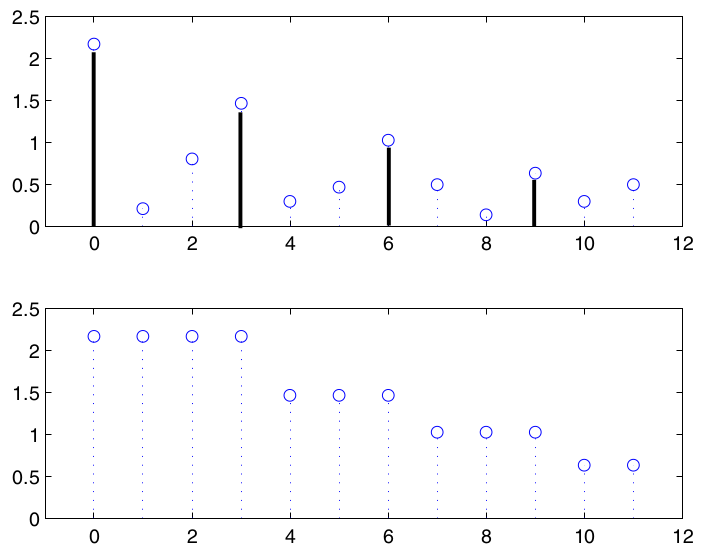
\includegraphics[width=0.5\linewidth]{nonmonotone}
	\caption{The sequences $\{f(x_k)\}_k$ and $\{R_k\}_k$.}
\end{figure}
\begin{theorem}
	Let $f\in \C(\Rn)$ be a globally Lipschitz continuous function, limited from below. Let $\{x_k\}_k$ be a sequence generated by Algorithm \ref{alg:gd_armijo} for solving $\min_{x\in\Rn}\;f(x)$, where \eqref{eq:grippo} is used instead of \eqref{eq:armijo}. Then we have 
	\begin{itemize}
		\item[(a)] $x_k \in \mathcal{L}_0 \;\;\forall k$ (where $\mathcal{L}_0:=\{x\in\Rn: f(x)\leq f(x_0)\}$)
		\item[(b)] $\displaystyle\lim_{k \to \infty} R_k = \displaystyle\lim_{k \to \infty} f(x_k) = f^*$ 
		\item[(c)] $\displaystyle\lim_{k \to \infty} t_k \grad(x_k) = 0$ as $k\to \infty$.
	\end{itemize}
\end{theorem}
\begin{proof}
	First, we show that the sequence $\{R_k\}_k$ is monotonically nonincreasing. For each $k,$ let \\
	$r(k)\in[k-\min\{k,M\}, k]$ be the smallest integer such that 
\begin{equation*}
	R_k = f(x_{r(k)})=\max_{0\leq j \leq \min\{k,M\}} f(x_{k-j}).
\end{equation*}
Thus, we rewrite \eqref{eq:armijo} as
	\begin{equation}\label{eq:lemma_condition}
		f(x_{k+1}) \leq f(x_{r(k)}) - \alpha t_k \| \grad(x_k)\|^2 = f(x_{r(k)}) - \frac{\alpha}{t_k} \| x_{k+1} -x_k \|^2,
	\end{equation}
	Since min$(k+1, M) \leq $ min$(k, M) +1$, we have
	\begin{equation*}
		\begin{split}
			f(x_{r(k+1)}) &= \displaystyle \max_{0 \leq j \leq \text{min}(k+1, M)} f(x_{k-j+1})\\
			& \leq \displaystyle \max_{0 \leq j \leq \text{min}(k, M) +1} f(x_{k-j+1})\\
			& = \displaystyle \max \{ f(x_{r(k)}), f(x_{k+1})\} = f(x_{r(k)}),
		\end{split}
	\end{equation*}
	where last equality follows from (\ref{eq:lemma_condition}). Since $\{f(x_{r(k)})\}$ is nonincreasing and $x_{r(0)} = x_{0}$, we have that $f(x_k) \leq f(x^0) \; \forall k$, which proves $(a)$.
	\par Since $f$ is limited from below, the monotone nonincreasing sequence $\{f(x_{r(k)})\}$ admits a limit $f^*$ for $k \to \infty$. By induction on $j$, with $1\leq j \leq M+1$, let us prove that the two limits below are satisfied:
	\begin{eqnarray}
		\displaystyle \lim_{k \to \infty} \| x_{r(k) -j +1} -x_{r(k)-j}\| = 0 \label{eq:induction1}\\
		\displaystyle \lim_{k \to \infty} f(x_{r(k) -j}) = \displaystyle \lim_{k\to \infty} f(x_{r(k)}) \label{eq:induction2}
	\end{eqnarray}
	where $k$ is assumed to be large enough to have $r(k) \geq k -M >1.$
	\par If $j=1$, using $(\ref{eq:lemma_condition})$ with $k = r(k) - 1$, we have
	\begin{equation*}
		f(x_{r(k)}) \leq f(x_{r(r(k)-1)}) - \frac{\alpha}{t_{r(k)-1}}\| x_{r(k)} - x_{r(k)-1}\|^2.
	\end{equation*}
	Thus, together with convergence of $\{f(x_{r(k)})\}$ and the fact that $t_k\leq s$, we obtain 
	$$ \displaystyle \lim_{k \to \infty} \| x_{r(k)} -x_{r(k)-1}\| = 0$$
	From Lipschitz continuity of $f$ and the above limit we obtain that
	\begin{equation*}
		\displaystyle \lim_{k\to\infty} f(x_{r(k) -1}) = \displaystyle \lim_{k\to\infty} f(x_{r(k) }),
	\end{equation*}
	which means that induction has been proved for the case $j=1$.
	\par Now assume that (\ref{eq:induction1}) and (\ref{eq:induction2}) are valid for a given $j$. From (\ref{eq:lemma_condition}) used with\\ $k = r(k) -j -1$, we have that
	$$ f(x_{r(k) -j}) \leq f(x_{r(r(k)-j -1)}) - \frac{\alpha}{t_{r(k)-j-1}}\| x_{r(k)-j} - x_{r(k)-j-1}\|^2.$$
	Thus, together with (\ref{eq:induction2}), where the left limit is used for the LHS and the right limit is used for the RHS and remembering that $k=  r(k) -j -1$, and that $t_k\leq s$ we obtain that
	$$ \displaystyle \lim_{k \to \infty} \| x_{r(k)-j} - x_{r(k)-j-1} \| = 0,$$
	which means that \eqref{eq:induction1} holds for $j+1$.	From the limit above, Lipschitz continuity of $f$ and again (\ref{eq:induction2}) we obtain that
	\begin{equation*}
		\displaystyle \lim_{k\to\infty} f(x_{r(k)-j-1}) =\displaystyle \lim_{k\to\infty} f(x_{r(k)-j})  = \displaystyle \lim_{k\to\infty} f(x_{r(k)}), 
	\end{equation*}
	which means that induction has been proved from a generic $j$ to $j+1$.
	\par Let us rewrite $x_{r(k)}$ as follows 
	\begin{equation} \label{eq:xk_to_xRk}
		\begin{split}
			x_{r(k)} &= x_k + (x_{k-1} - x_k) + \dots +(x_{r(k)} - x_{r(k)+1})\\
			%&= x_k + \sum_{j=1}^{k-r(k)} \left (x_{k-j} - x_{k-j+1} \right )\\
			&= x_k + \sum_{j=1}^{k-r(k)} \left (x_{r(k) +j-1} - x_{r(k)+j} \right ).
		\end{split}
	\end{equation}
	In order to apply \eqref{eq:induction1} on each of the terms of sum in \eqref{eq:xk_to_xRk}, we first have to notice that they are $k-r(k)  \leq M$ consecutive terms, meaning that there exists a future $k'$ and corresponding $r(k')\geq k$ such that
	$$\sum_{j=1}^{k-r(k)} \left (x_{r(k) +j-1} - x_{r(k)+j} \right ) = - \sum_{j=r(k')-k+1}^{r(k')-r(k)} x_{r(k') -j+1} - x_{r(k')-j}.$$
    Notice that $r(k')-r(k)\geq r(k')-k+1 \geq 1$ and that $r(k')-r(k) - (r(k')-k+1)\leq M$, meaning that we can apply \eqref{eq:induction1} on the terms of the RHS of the above equality to get, together with \eqref{eq:xk_to_xRk}, the following
	\begin{equation*}
		\displaystyle \lim_{k\to \infty} \| x_k - x_{r(k)}\| = 0.
	\end{equation*}
	From the above limit and the Lipschitz continuity of $f$ (plus the fact that the sequence of $\{f(x_{r(k)})\}$ converges to $f^*$), it follows that
	$$ \displaystyle\lim_{k\to \infty} f(x_k) = \displaystyle\lim_{k\to \infty}  f(x_{r(k)})= f^*,$$
	which completes the proof of $(b)$. Thesis $(c)$ follows from $(b)$ and \eqref{eq:lemma_condition}. 
\end{proof}
To achieve the asymptotic convergence to stationary points for this method, we can use Theorem \ref{thm:Armijo_convergence_p2} by noticing that \eqref{eq:failure} can be achieved also for \eqref{eq:grippo}, as the additional value $R_k-f(x_k)$ is positive and can be thus neglected.

\begin{theorem}
	Algorithm \ref{alg:gd_armijo} applied to minimize a function $f\in \LC(\Rn)$ bounded from below may require as many as $\epsilon^{-2}$ evaluations of $f$ and $\grad$ to produce an iterate $x\in \Rn$ such that $||\grad (x)\|\leq \epsilon.$
\end{theorem}
\noindent The proof of this theorem is out of the scope of this course, see the proof of Theorem 2.2.3 from \cite{cartis22a}.

\section{Gradient method on convex functions}
In the following 3 sections, we will see how to speed up the convergence of GD for functions with additional structure. In particular, we will cover convex functions, strongly convex functions and functions satisfying the Polyak-\L ojasiewicz condition. Moreover, we will simplify the analysis by assuming $f\in \LC(\Rn)$.
\begin{definition}[Convex Function]
	A function $f:\Rn\to \R$ is said to be convex if given $x_1,x_2\in \Rn$ and $\lambda\in [0,1]$, then 
	\begin{equation*}
		f(\lambda x_1 +(1-\lambda) x_2) \leq \lambda f(x_1) +(1-\lambda) f(x_2).
	\end{equation*}
\end{definition}
\begin{definition}[Strictly Convex Function]
	A function $f:\Rn\to \R$ is said to be strictly convex if given $x_1,x_2\in \Rn$ and $\lambda\in [0,1]$, then 
	\begin{equation*}
		f(\lambda x_1 +(1-\lambda) x_2) < \lambda f(x_1) +(1-\lambda) f(x_2).
	\end{equation*}
\end{definition}

\noindent A function is called concave if $-f$ is convex and strictly concave if $-f$ is strictly convex.\\
Now, given $\Delta_k$ the unit-simplex, that is the
subset of $\R^k$ comprising all nonnegative vectors whose sum is 1, i.e., 
\begin{equation*}
	\{\lambda \in \R^k: \lambda\geq 0, e^t\lambda=1\},
\end{equation*}
we can provide the following very useful result by Jensen's.
\begin{theorem}[Jensen's Inequality]
	Let $f:\Rn\to \R$ be a convex function. Then for any $x_1, x_2, \dots, x_k \in \Rn$ and $\lambda\in \Delta_k$ we have
	\begin{equation}\label{eq:jensen}
		f\left(\sum_{i=1}^{k}\lambda_ix_i\right) \leq \sum_{i=1}^{k} \lambda_if(x_i).
	\end{equation}
\end{theorem}
\begin{proof}
	We will prove \eqref{eq:jensen} by induction on $k$. For $k=1$ the result is obvious ($f(x_1)\leq f(x_1)\;\;\forall x_1 \in \Rn$). We now assume that \eqref{eq:jensen} holds for $k$ and we will prove that it also holds for $k+1$. Suppose we have $x_1, x_2, \dots, x_{k+1} \in \Rn$ and $\lambda\in \Delta_{k+1}$, we will show that $f(z)\leq \sum_{i=1}^{k+1} \lambda_i f(x_i)$ with $z=\sum_{i=1}^{k+1} \lambda_i x_i$. If $\lambda_{k+1} =1$, then $z=x_{k+1}$ and \eqref{eq:jensen} is obvious. If $\lambda_{k+1}<1$, then
	\begin{equation*}
		\begin{split}
			f(z)& = f\left(\sum_{i=1}^k \lambda_i x_i + \lambda_{k+1}x_{k+1} \right)\\
			&= f\left((1-\lambda_{k+1})\sum_{i=1}^k \frac{\lambda_i}{1-\lambda_{k+1}} x_i + \lambda_{k+1}x_{k+1} \right)\\
			&\leq (1-\lambda_{k+1})f(v) + \lambda_{k+1} f(x_{k+1}),
		\end{split}
	\end{equation*}
	with $v= \sum_{i=1}^k\frac{\lambda_i}{1-\lambda_{k+1}} x_i$ where the last inequality follows by convexity. Since $\sum_{i=1}^k\frac{\lambda_i}{1-\lambda_{k+1}} = \frac{1-\lambda_{k+1}}{1-\lambda_{k+1}} = 1,$ it follows that $v$ is a convex combination of $k$ points from $\Rn$, hence by the induction hypotesis we have that $f(v)\leq \sum_{i=1}^k\frac{\lambda_i}{1-\lambda_{k+1}} f(x_i)$, which combined with the equality above yields
	\begin{equation*}
		f(z) \leq \sum_{i=1}^{k+1} \lambda_i f(x_i).
	\end{equation*}
\end{proof}
\begin{theorem}[Gradient characterization of convex functions]\label{thm:gradient_ineq}
	Let $f\in \C(\Rn)$. Then f is convex over $\Rn$ if and only if
	\begin{equation}\label{eq:grad_ineq}
		f(x) +\grad(x)^T(y-x)\leq f(y) \quad \forall x, y\in \Rn.
	\end{equation}
\end{theorem}
\begin{proof}
	Exercise.
\end{proof}
\begin{proposition}[Sufficiency of stationarity under convexity]\label{prop:stationarity}
	Let $f\in \C(\Rn)$ be a convex function. Suppose that $\grad(x^*)=0$ for some $x^*\in \Rn$. Then $x^*$ is a global minimizer of $f$ over $\Rn$.
\end{proposition}
\begin{proof}
	Let $z\in \Rn$. Plugging $x=x^*$ and $y=z$ in Theorem \ref{thm:gradient_ineq} we obtain that 
	\begin{equation*}
		f(z)\geq f(x^*) +\grad(x^*)^T(z-x^*),
	\end{equation*}
	which implies that $f(z)\geq f(x^*) $ because $\grad(x^*)=0$.
\end{proof}
In particular when $f$ is convex, being a stationary point is both sufficient and necessary condition for $x^*$ to be a global minimum.
We can now establish the conditions under which a twice continuously differentiable function $f$ is convex.
\begin{theorem}[Second order characterization of convexity]
	Let $f\in \Cii(\Rn)$. Thus, we have that $f$ is convex iff $\hess(x)\succcurlyeq0\quad \forall x\in \Rn.$
\end{theorem}
\begin{proof}
	Suppose that $\hess(x) \succcurlyeq 0$ for all $x \in \Rn$. We will prove \eqref{eq:grad_ineq} which is enough to establish convexity. Let $x,y\in \Rn$, then by the Mean Value Theorem$^2$ (Theorem 2.6 from Chapter 1) we get that there exists $z\in[x,y]$ for which 
	\begin{equation}\label{eq:mvt2_app}
		f(y) = f(x)+ \grad (x)^T(y-x) +\frac{1}{2}(y-x)^T\hess(z)(y-x).
	\end{equation}
	Since $\hess(z) \succcurlyeq 0$, it follows that $(y-x)^T\hess(z)(y-x)\geq0$, which implies \eqref{eq:grad_ineq}.
	To prove the opposite direction, assume that $f$ is convex. Let $x\in \Rn$ and $y\in \Rn$. Since $\Rn$ is open, it follows that $x+\lambda y \in \Rn$, for $0<\lambda<\epsilon$, where $\epsilon$ is a small enough positive constant. Using now the gradient characterization of convex functions \eqref{eq:grad_ineq} we get 
	\begin{equation*}
		f(x+\lambda y) \geq f(x) + \lambda\grad(x)^Ty.
	\end{equation*}
	In addition, by the quadratic approximation theorem (Theorem 2.4 from Chapter 1), we have that 
	\begin{equation*}
		f(x+\lambda y) = f(x) + \lambda \grad(x)^Ty + \frac{\lambda^2}{2}y^T\hess(x)y + o(\lambda^2||y||^2),
	\end{equation*}
	which combined with the above inequality gives 
	\begin{equation*}
		\frac{\lambda^2}{2}y^T\hess(x)y + o(\lambda^2||y||^2) \geq 0 \quad \forall \lambda\in (0,\epsilon).
	\end{equation*}
	Dividing the latter inequality by $\lambda^2$ and taking the limit for $\lambda\to 0^+$, we have 
	\begin{equation*}
		y^T\hess(x)y \geq 0 \quad \forall y \in \Rn,
	\end{equation*}
	which concludes the proof.
\end{proof}
The same theorem works with positive definiteness and strict convexity, meaning also that the minimum in this case is unique.\\
In order to prove an enhanced rate of convergence for GD on convex functions, we need the following lemma.
\begin{lemma}[Co-coercivity]
	Let $f\in \LC(\Rn)$ be convex, then $\forall x, y \in \Rn$ we have both
	\begin{align}
		\frac{1}{2L} ||\grad(y)-\grad(x)||^2 \leq f(y)-f(x) -\grad(x)^T(y-x)\label{eq:pre_cocoercivity}\\
		\frac{1}{L} ||\grad(y)-\grad(x)||^2 \leq (\grad(y)-\grad(x))^T(y-x)\label{eq:cocoercivity}
	\end{align}
\end{lemma}
\begin{proof}
	By employing \eqref{eq:grad_ineq} and the Descent Lemma (part 1), we get
	\begin{equation*}
		\begin{split}
			f(x) - f(y) &= f(x) - f(z) + f(z) - f(y)\\
			& \leq \grad(x)^T(x-z) + f(z) - f(y)\\
			&\leq \grad(x)^T(x-z) + \grad(y)^T(z-y) + \frac{L}{2}||z-y||^2=:g(z)
		\end{split}
	\end{equation*}
To get the tightest upper bound on the RHS, we can minimize $g(z)$ w.r.t. $z$ by looking for a stationary point, i.e., $\nabla g(z)=0$, from which we get $z=y - \frac{1}{L}(\grad(y)-\grad(x))$. Notice that this stationary point is a global minimum of $g(z)$ because this function is convex in $z$. By replacing this $z$ in the inequality above, we get 
\begin{equation*}
	\begin{split}
		f(x) - f(y) &\leq \grad(x)^T(x-y) -\frac{1}{L}||\grad(y)-\grad(x)||^2 + \frac{1}{2L}||\grad(y)-\grad(x)||^2\\
		&= \grad(x)^T(x-y)-\frac{1}{2L}||\grad(y)-\grad(x)||^2,
	\end{split}
\end{equation*}
which proves \eqref{eq:pre_cocoercivity}. To obtain \eqref{eq:cocoercivity} we apply \eqref{eq:pre_cocoercivity} twice by interchanging the role of $x$ and $y$
\begin{align*}
	\frac{1}{2L} ||\grad(y)-\grad(x)||^2 \leq f(y)-f(x) -\grad(x)^T(y-x)\\
	\frac{1}{2L} ||\grad(y)-\grad(x)||^2 \leq f(x)-f(y) -\grad(y)^T(x-y),
\end{align*}
and sum those last two inequalities.
\end{proof}
\noindent For simplicity, we will assume to know $L$, so that we can employ Algorithm \eqref{gd}, i.e. $t=\frac{1}{L}$.
\begin{theorem}[Rate of Convergence of GD for Convex Functions]
	Let $f\in \LC(\Rn)$ be convex and let $\{x_k\}$ be a sequence generated by Algorithm \ref{gd}. Assume that there exists $x^*\in \argmin f(x)$, with corresponding value $f^*=f(x^*)$, then we have 
	\begin{equation}\label{eq:convex_convergence}
		f(x_T)-f^* \leq \frac{L ||x_0-x^*||^2}{2T}.
	\end{equation}
\end{theorem}
\begin{proof}
	Let $f$ be convex and $L$-smooth. From \eqref{eq:cocoercivity} applied on $y=x_k$ and $x=x^*$, and remembering that $x^*$ is a stationary point, it follows that
	\begin{align*}
		\|x_{k+1} - x^*\|^2 &= \|x_k - x^* - \frac{1}{L}\grad(x_k)\|^2\\
		&= \|x_k - x^*\|^2 - \frac{2}{L} \grad(x_k)^T(x_k - x^*) + \frac{1}{L^2}\|\grad(x_k)\|^2\\
		&\leq \|x_k - x^*\|^2 - \frac{1}{L^2}\|\grad(x_k)\|^2.
	\end{align*}
	Thus, $\|x_k - x^*\|^2$ is a non-increasing sequence, from which we get 
	\begin{align}\label{eq:23}
		\|x_k - x^*\| \leq \|x^0 - x^*\|.
	\end{align}
	From \eqref{eq:decrease} and subtracting $f(x^*)$ from both sides, we have
	\begin{align}\label{eq:24}
		f(x_{k+1}) - f(x^*) \leq f(x_k) - f(x^*) - \frac{1}{2L}\|\grad(x_k)\|^2.
	\end{align}
	Applying convexity, Cauchy-Schwartz and \eqref{eq:23}, we have that
	\begin{equation*}
		\begin{split}
			f(x_k) - f(x^*) &\leq \grad(x_k)^T(x_k - x^*)\\
			&\leq \|\grad(x_k)\|\|x_k - x^*\| \leq \|\grad(x_k)\|\|x^0 - x^*\|.
		\end{split}
	\end{equation*}
	Isolating $\|\grad(x_k)\|$ in the above inequality and inserting it in \eqref{eq:24} gives
	\begin{equation*}
		f(x_{k+1}) - f(x^*) \leq f(x_k) - f(x^*) - \frac{1}{2L}\frac{1}{\|x^0 - x^*\|^2}(f(x_k) - f(x^*))^2
	\end{equation*}
	Let $\delta_k = f(x_k) - f(x^*)$ and $\gamma:=\frac{1}{2L||x_0-x^*||^2}$. Since $\delta_{t+1} \leq \delta_k$, and by manipulating the inequality above we have that
	\begin{align*}
		\delta_{t+1} \leq \delta_k - \gamma\delta_k^2 \overset{\cdot\frac{1}{\delta_k\delta_{k+1}}}{\Rightarrow} \gamma\frac{\delta_k}{\delta_{k+1}} \leq \frac{1}{\delta_{k+1}} - \frac{1}{\delta_k} \overset{\delta_{k+1}\leq\delta_k}{\Leftrightarrow} \gamma \leq \frac{1}{\delta_{k+1}} - \frac{1}{\delta_k}.
	\end{align*}
	Summing up both sides over $k = 0, \ldots, T - 1$ and using telescopic cancellation we have that
	\begin{align*}
		T\gamma \leq \frac{1}{\delta_T} - \frac{1}{\delta_0} \leq \frac{1}{\delta_T}.
	\end{align*}
Re-arranging the above we have that
	\begin{align*}
		f(x_T) - f(x^*) = \delta_T \leq \frac{1}{\gamma T} = \frac{2L\|x^0 - x^*\|^2}{T}.
	\end{align*}
\end{proof}

Notice that by \eqref{eq:pre_cocoercivity} applied on $y=x$ and $x=x^*$, we have $ \frac{1}{2L}\|\grad(x) \|^2 \leq f(x)-f^*$, meaning that the actual termination criterion of Algorithm \ref{gd} on the norm of the gradient also works for convex functions. In particular, we have the following.
\begin{corollary}
	The iteration complexity of Algorithm \eqref{gd} on convex functions is $\BigO(\epsilon^{-1})$.
\end{corollary}
\begin{proof}
	Exercise, express the constants of the $\BigO(\epsilon^{-1})$.
\end{proof}

\section{Gradient method on strongly convex functions}

\begin{definition}[Strongly Convex Function]
	Let $f : \Rn \to \R$, and $\mu > 0$. We say that $f$ is $\mu$-strongly convex if, for every $x, y \in \Rn$, and every $\lambda \in [0, 1]$ we have that
	\begin{equation*}
		\mu \frac{\lambda(1-\lambda)}{2} \|x - y\|^2 + f(\lambda x + (1-\lambda)y) \leq \lambda f(x) + (1-\lambda)f(y).
	\end{equation*}
We say that $\mu$ is the strong convexity constant of $f$.
\end{definition}
The term $ \mu\|x - y\|^2$ ensures that when moving away from $x$ the function value grows at least as a quadratic with curvature $\mu$. In fact, a strongly convex function has at least a quadratic growth with curvature $\mu$ at any point, in other words, there are no flat regions. This has a very positive effect on the speed of convergence of GD. \\



The lemma below shows that it is easy to craft a strongly convex function: just add a multiple of $\| \cdot \|^2$ to a convex function. This happens for instance when using Tikhonov regularization (a.k.a. ridge/$\ell_2$ regularization) in machine learning or inverse problems.

\begin{lemma}\label{lemma:l2_regularization}
	Let $f : \Rn \to \R$, and $\mu > 0$. The function $f$ is $\mu$-strongly convex if and only if there exists a convex function $g : \Rn \to \R$ such that $f(x) = g(x) + \frac{\mu}{2}\|x\|^2$.
\end{lemma} 
\begin{proof}
	Given $f$ and $\mu$, define $g(x) := f(x) - \frac{\mu}{2}\|x\|^2$. We need to prove that $f$ is $\mu$-strongly convex if and only if $g$ is convex. By denoting $z_\lambda := (1-\lambda)x + \lambda y$,  $f$ is $\mu$-strongly convex
	\begin{align*}
		&\Leftrightarrow f(z_\lambda) + \frac{\mu}{2}\lambda(1-\lambda)\|x - y\|^2 \leq (1-\lambda)f(x) + \lambda f(y) \quad \forall \lambda \forall x, y\in \Rn \\
		&\Leftrightarrow g(z_\lambda) + \frac{\mu}{2}\|z_\lambda\|^2 + \frac{\mu}{2}\lambda(1-\lambda)\|x - y\|^2 \leq (1-\lambda)g(x) + \lambda g(y) + (1-\lambda)\frac{\mu}{2}\|x\|^2 + \lambda\frac{\mu}{2}\|y\|^2 \quad \forall \lambda \forall x, y\in \Rn.
	\end{align*}
	Let us now gather all the terms multiplied by $\mu$ to find that
	\begin{align*}
		&\frac{1}{2}\|z_\lambda\|^2 + \frac{1}{2}\lambda(1-\lambda)\|x - y\|^2 - (1-\lambda)\frac{1}{2}\|x\|^2 - \lambda\frac{1}{2}\|y\|^2 \\
		&= (1-\lambda)^2\|x\|^2 + \lambda^2\|y\|^2 + 2\lambda(1-\lambda) x^Ty + \lambda(1-\lambda)\|x\|^2 + \lambda(1-\lambda)\|y\|^2 - 2\lambda(1-\lambda) x^Ty\\
		&\quad - (1-\lambda)\|x\|^2 - \lambda\|y\|^2 \\
		&= \|x\|^2\left((1-\lambda)^2 + \lambda(1-\lambda) - (1-\lambda)\right) + \|y\|^2\left(\lambda^2 + \lambda(1-\lambda) - \lambda\right) \\
		&= 0.
	\end{align*}
	
	\noindent Thus, all the terms in $\mu$ disappear, and what remains is exactly the definition for $g$ to be convex.
\end{proof}

\noindent Let us now present some useful lemmas, that can be proved by exploiting Lemma \ref{lemma:l2_regularization}.
\begin{lemma}
	Let $f : \Rn \to \R$ be continuous and strongly convex, then $f$ admits a unique minimizer.
\end{lemma}
\begin{proof}
	Exercise. The existence of $x^*$ follows from the coercivity of $f$.
\end{proof}

\begin{lemma}
	Let $f \in \C(\Rn)$ be $\mu$-strongly convex, then
	\begin{equation}\label{eq:variational_sc}
		\text{for all } x, y \in \Rn, \quad f(y) \geq f(x) + \grad(x)^T(y - x) + \frac{\mu}{2}\|y - x\|^2.
	\end{equation}
\end{lemma}

\begin{proof}
	Exercise.
%	Define $g(x) := f(x) - \frac{\mu}{2}\|x\|^2$. According to Lemma 2.12, $g$ is convex. It is also clearly differentiable by definition. According to the sum rule, we have $\grad(x) = \nabla g(x) + \mu x$. Therefore we can use the convexity of $g$ with Definition 8.4 to write
%	\begin{equation}
%		f(y) - f(x) - \langle \grad(x), y - x \rangle \geq \frac{\mu}{2}\|y\|^2 - \frac{\mu}{2}\|x\|^2 - \langle \mu x, y - x \rangle = \frac{\mu}{2}\|y - x\|^2.
%	\end{equation}
\end{proof} 

\begin{lemma}Let $f\in \Cii(\Rn)$ be $\mu$-strongly convex. Then, for all $x \in \Rn$, for every eigenvalue $\lambda$ of $\nabla^2 f(x)$, we have $\lambda \geq \mu$.\\
	Moreover, if $f\in \LC(\Rn)$, for every eigenvalue $\lambda$ of $\nabla^2 f(x)$, we have $\lambda \leq L$, i.e., $L \cdot \Id\succcurlyeq\hess(x)\succcurlyeq\mu \cdot\Id$
\end{lemma}

\begin{proof}
	Exercise.
%	Define $g(x) := f(x) - \frac{\mu}{2}\|x\|^2$, which is convex according to Lemma 2.12. It is also twice differentiable, by definition, and we have $\nabla^2 f(x) = \nabla^2 g(x) + \mu I d$. So the eigenvalues of $\nabla^2 f(x)$ are equal to the ones of $\nabla^2 g(x)$ plus $\mu$. We can conclude by using Lemma 2.9. 
\end{proof}

%\begin{example}[Least-squares and strong convexity]
%	Let $f$ be a least-squares function as in Exercise 2.10. Then $f$ is strongly convex if and only if $\Phi$ is injective. In this case, the strong convexity constant $\mu$ is $\lambda_{\min}(\Phi^{\top} \Phi)$, the smallest eigenvalue of $\Phi^{\top} \Phi$.
%\end{example}

\begin{theorem}[Rate of Convergence of GD for Strongly Convex Functions]\label{thm:strongly_convex}
	Let $f\in \LC(\Rn)$ be strongly convex and let $\{x_k\}$ be a sequence generated by Algorithm \ref{gd} with a step size $0<t\leq\frac{1}{L}$. Let $x^*= \argmin f(x)$, with corresponding value $f^*=f(x^*)$, then we have 
	\begin{equation}\label{eq:strongly_convex_convergence}
		\|x_T - x^*\|^2 \leq (1 - t\mu)^T\|x_0 - x^*\|^2.
	\end{equation}
\end{theorem}
\begin{proof}
	Since $f$ is strongly convex, it is also convex, thus we can apply \eqref{eq:pre_cocoercivity} on $y=x$ and $x=x^*$ to get
	\begin{equation}\label{eq:polyak_lb}
		\frac{1}{2L}\|\grad(x) \|^2 \leq f(x)-f^*
	\end{equation}
Thus, by applying \eqref{eq:polyak_lb} and \eqref{eq:variational_sc} with $x=x_k$ and $y=x^*$, we get 
\begin{align*}
	\|x_{k+1} - x^*\|^2 &= \|x_k - x^* - t\grad(x_k)\|^2\\
	&= \|x_k - x^*\|^2 - 2t \grad(x_k)^T (x_k - x^*) + t^2\|\grad(x_k)\|^2\\
	&\stackrel{\eqref{eq:variational_sc}}{\leq} (1-t\mu)\|x_k - x^*\|^2 - 2t(f(x_k) - f^*) + t^2\|\grad(x_k)\|^2\\
	&\stackrel{\eqref{eq:polyak_lb}}{\leq} (1-t\mu)\|x_k - x^*\|^2 - 2t(f(x_k) - f^*) + 2t^2 L(f(x_k) - f^*)\\
	&= (1-t\mu)\|x_k - x^*\|^2 - 2t(1 - t L)(f(x_k) - f^*). \tag{29}
\end{align*}
Since $\frac{1}{L} \geq t$ we have that $-2t(1 - t L)$ is negative, and thus can be safely dropped to give
\begin{equation*}
	\|x_{k+1} - x^*\|^2 \leq (1 - t\mu)\|x_k - x^*\|^2.
\end{equation*}
It now remains to unroll the recurrence till iteration $T-1$.
\end{proof}
\begin{corollary}
The iteration complexity of Algorithm \eqref{gd} on strongly convex functions is $\BigO(\log(\epsilon^{-1}))$.
\end{corollary}
\begin{proof}
Exercise.
\end{proof}
\begin{remark}
	The speed of convergence in Theorem \ref{thm:strongly_convex} is also called linear because... 
\end{remark}

\section{Gradient method on functions satisfying Polyak \L ojasiewicz}
\begin{definition}[Polyak \L ojasiewicz (PL) functions] Let $f\in \C(\Rn)$ and $\mu>0$. Than $f$ satisfies PL if it is bounded from below by $f^*=\inf f$ and $\forall x\in \Rn$ we have 
\begin{equation}\label{eq:pl}
	f(x) - f^* \leq \frac{1}{2\mu} ||\grad(x)||^2.
\end{equation}
\end{definition}
\noindent For a function satisfying the PL condition, the gradient provides a reliable signal about how far you are from optimality. In fact, the optimality gap $f(x) - f^*$ is dominated by the norm of the gradient, in other words, by minimizing the norm of the gradient, the iterates necessarily approach a global minimum. On the other side, if the iterates are far away from a minimizer, the norm of the gradient must be nonzero. 
\begin{lemma}
	Let $f\in \C(\Rn)$ satisfy PL. $x^*$ is a global minimizer if and only if $\grad(x^*)=0$.
\end{lemma}
\begin{proof}
	Follows directly from \eqref{eq:pl}.
\end{proof}
\noindent The PL property is weaker than strong convexity, as we see next.
\begin{lemma}
	Let $f\in \C^1(\Rn)$ and $\mu>0$. If $f$ is strongly convex, than $f$ satisfies $\mu$-PL.
\end{lemma}
\begin{proof}
	Exercise.
\end{proof}
It is important to note that the Polyak-Lojasiewicz property can hold without strong convexity
or even convexity, e.g., $f(t)=t^2+3\sin(t)^2$.\\
One must keep in mind that the PL property is rather strong, as it is a global property and
requires the following to be true, which is typical of convexity.
\begin{remark}
	PL can be extended in different ways. Some examples are given below:
	\begin{itemize}
		\item The inequality can be localized, by dropping the property that every critical point is
		a global minimum. To achieve this, we do not look at the growth of $f(x)-f(x^*)$, but at $f(x)-f(x^*)$
		instead, where $x^*\in \Rn$ is a critical point of interest. This can be written as 
		$$ f(x)-f(x^*)\leq \frac{1}{q\mu}\|\grad(x)\|^q \quad  \with \frac{1}{q}+\frac{1}{p}=1, \forall x\in \Omega$$
		There is a result (Corollary 16 from \cite{bolte07a}) showing that any semi-algebraic function (e.g., sums/products/min/max of polynomials) verifies the above inequality at every $x^* \in \Rn$ for some $p\geq 1, \mu > 0$, and $\Omega$ being an appropriate neighborhood of $x^*$. This framework includes for instance quadratic losses evaluating a Neural Network with ReLU as activations.
		\item In order to deal with different kind of growth between the norm of the gradient and the decrease of the function values. In particular, there exists a more general property called Kurdyka-\L ojasiewicz (K\L). A differentiable function $f:\Rn\to\R$ satisfies K\L $\,$ on $S\subset \Rn$, if for every $x^*\in S$, there exists a neighborhood $B(x^*,r)$ with $r>0$ and a function $\phi \in \Phi_\xi$ such that 
		$$||\grad(x)|| \phi'(f(x) - f(x^*) \geq 1 \quad \forall x \in B(x^*,r) \text{ satisfying } 0<f(x)-f(x^*)<\xi,$$
		where for every $\xi>0$, we denote by $\Phi_\xi$ the set of concave functions $\phi:[0,\xi)\to\R_+$ such that $\phi(0)=0$, $\phi\in \C([0,\xi))$ and $\phi'(s)>0 \quad \forall s\in (0,\xi)$. 
	\end{itemize}
\end{remark}

\begin{theorem}[Rate of Convergence of GD under PL]\label{thm:pl_convergence}
	Let $f\in \LC(\Rn)$ satisfy $\mu$-PL for some $L\geq \mu >0$ and let $\{x_k\}$ be a sequence generated by Algorithm \ref{gd} with a step size $0<t\leq\frac{1}{L}$. Then we have 
	\begin{equation}\label{eq:pl_convergence}
		f(x_T)-f^*\leq (1-t\mu)^T(f(x_0)-f^*)
	\end{equation}
\end{theorem}
\begin{proof}
	From the Descent Lemma (part 2), $tL<1$, and the PL property we get 
	\begin{align*}
			f(x_{k+1}) &\leq f(x_k) - t(1-\frac{Lt}{2})||\grad(x_k)\|^2\\
			& \leq f(x_k) -\frac{t}{2}||\grad(x_k)\|^2\\
			& \leq f(x_k) - t\mu (f(x_k)-f^*).
	\end{align*}
Thus, by subtracting $f^*$ on both sides, on the LHS we have $(1-t\mu)(f(x_k)-f^*)$, and by recursion until $T-1$ we get the thesis.
\end{proof}
\begin{corollary}
The iteration complexity of Algorithm \eqref{gd} on functions satisfying PL is $\BigO(\log(\epsilon^{-1}))$.
\end{corollary}
\begin{proof}
Exercise.
\end{proof}

\section{Barzilai-Borwein Method}
%\subsubsection{The Quadratic Case}
Let us first consider a quadratic objective function, 
\begin{equation}\label{eq:quadratic}
	f(x) = x^TQx + c^Tx + b,
\end{equation}
where $x,c\in\Rn$, $b\in \R$, $Q\in \Rnn$ is symmetric and positive definite. In this case, we get the following result for GD.
\begin{proposition}[Finite convergence of GD in the quadratic case]
	Let $\lambda_1\geq \lambda_2, \dots,\lambda_n$ be the eigenvalue of the Hessian of the quadratic function \eqref{eq:quadratic}. Then, GD defined by the iteration
	\begin{equation}\label{eq:eigengrad}
		x_{k+1} = x_k -\frac{1}{\lambda_k} \grad(x_k) \quad \with k=1, \dots, n,
	\end{equation}
	determines in at maximum $n$ iterations the minimizer of $x_k$. 
\end{proposition}
\begin{proof}
	As gradient of \eqref{eq:quadratic} is $\grad(x)=Qx+c$, we get
	\begin{equation*}
		\grad(x_{k+1}) = Qx_{k+1} +c = Qx_k +c -\frac{1}{\lambda_k} Q \grad(x_k) = \left(I -\frac{1}{\lambda_k}Q\right)\grad(x_k)
	\end{equation*}
Repeating the application of the above formula, we get 
\begin{equation*}
	\grad(x_k) = \left(\prod_{j=1}^{k-1}(I-\frac{1}{\lambda_j}Q)\right)\grad(x_1)
\end{equation*}
Let ${u_h \in \Rn: h=1, \dots, n}$ be the set of eigenvectors of $Q$, associated to the eigenvalues $\lambda_h$, in particular they form a basis of $\Rn$, meaning that we can represent $\grad(x_1)$ as a linear combination of these vectors, i.e.,  
\begin{equation*}
	\grad(x_1) = \sum_{h=1}^{n} \beta_h u_h,\quad\with \beta_h\in\R. 
\end{equation*}
Thus, for $k\geq 2$, we get 
\begin{equation*}
	\grad(x_k) = \left(\prod_{j=1}^{k-1}(I-\frac{1}{\lambda_j}Q)\right) \left(\sum_{h=1}^{n} \beta_h u_h\right),
\end{equation*}
and consequently, setting $k=n+1$, from $Iu_h = u_h$ and $Qu_h=\lambda_hu_h$, we have
\begin{equation*}
	\grad(x_{n+1}) = \sum_{h=1}^{n} \beta_h \left(\prod_{j=1}^{n}(1-\frac{1}{\lambda_j}\lambda_h)\right) u_h=0,
\end{equation*}
from which we get that GD converges in at most $n$ steps.
\end{proof}
Unfortunately, the eigenvalues of $Q$ are usually not available and obtaining them is roughly as expensive as applying $GD$ on \eqref{eq:quadratic}. For this reason we consider instead of \eqref{eq:eigengrad} to approximate them on the fly via the Rayleigh quotient
\begin{equation*}
	R_Q(x) := \frac{x^TQx}{||x||^2} \quad \forall x\neq 0,
\end{equation*}
given that 
\begin{equation*}
	\lambda_n(Q) \leq R_Q(x) \leq \lambda_1(Q) \quad \forall x\neq 0. 
\end{equation*}
In particular, if the image of $Q$ is small (i.e., the interval $[\lambda_n(Q),\lambda_1(Q)]$ is small), $R_Q(x)$ approximates the eigenvalues of $Q$. Moreover, we can compute $R_Q(x)$ without directly involving $Q$ if we select $x$ in a smart way. In particular, given two points $x,y\in\Rn,$ we get 
\begin{equation*}
	\grad(x) = Qx-c \quad \text{and}\quad \grad(y) = Qy-c \quad \Rightarrow \quad \grad(y) - \grad(x) = Q(y-x).
\end{equation*} 
Thus, with $x=x_{k-1}$ and $y=x_k$, and calling 
\begin{equation*}
	y_k:= \grad(x_k) - \grad(x_{k-1})  \quad \text{and} \quad s_k= x_k -x_{k-1}
\end{equation*}
we get $y_k = Qs_k$ and consequently
\begin{equation}\label{eq:railey_bb1}
	R_Q(s_k) = \frac{s_k^TQs_k}{||s_k||^2} =  \frac{s_k^Ty_k}{||s_k||^2}=: \mu_k^{BB1},
\end{equation}
where BB stands for Barzilai-Borwein method, but also $s_k=Q^{-1}y_k$ and consequently
\begin{equation*}
	R_{Q^{-1}}(y_k) = \frac{y_k^TQ^{-1}y_k}{||y_k||^2} =  \frac{s_k^Ty_k}{||y_k||^2}=: \mu_k^{BB2}.
\end{equation*}
Recalling \eqref{eq:eigengrad} we get two algorithms
\begin{equation}\label{eq:bb1}
	x_{k+1} = x_k -\frac{1}{\mu_k^{BB1}} \grad(x_k) 
\end{equation}
and 
\begin{equation}\label{eq:bb2}
	x_{k+1} = x_k -\frac{1}{\mu_k^{BB2}} \grad(x_k).
\end{equation}
In particular, for \eqref{eq:bb1}, and equivalently for \eqref{eq:bb2}, we get the following proposition.
\begin{proposition}
	Given $\{x_k\}_k$ the sequence generate by Algorithm \eqref{eq:bb1} to solve \eqref{eq:quadratic}, with $Q$ symmetric and positive definite, with $2\lambda_n>\lambda_1$, we get 
	\begin{equation*}
		\| \grad(x_k)\|\leq \delta^k \|\grad(x_0)\| \quad \with \delta=\frac{\lambda_n}{\lambda_1}-1.
	\end{equation*}
\end{proposition}
\begin{proof}
Exercise.
\end{proof}
\noindent Beyond this result, the same type of convergence (with a constant $\delta<1$) can be proved also without assuming $2\lambda_n>\lambda_1$. %TODO type of convergence


\subsection{Barzilai-Borwein in the Non-Quadratic Case}
In the non quadratic case, applying the fundamental theorem of calculus to $\grad(x)$, we get that
\begin{equation*}
\grad(x_k)=\grad(x_{k-1}) + \int_{0}^{1} \hess(x_k+t(x_k-x_{k-1})) (x_k-x_{k-1}) dt
\end{equation*} 
from which we can rewrite $\mu_k^{BB1}$ from \eqref{eq:railey_bb1} as
\begin{equation*}
	\mu_k^{BB1} = \frac{(\grad(x_k)-\grad(x_{k-1}))^T(x_k-x_{k-1})}{\|x_k - x_{k-1}\|^2} = \frac{\int_{0}^{1}(x_k-x_{k-1})^T \hess(x_k+t(x_k-x_{k-1})) (x_k-x_{k-1}) dt }{\|x_k - x_{k-1}\|^2}.
\end{equation*}
Thus, $\mu_k^{BB1}$ is the mean of the Rayleigh quotient over the Hessians computed on the segment $[x_k, x_{k-1}]$. On the other hand, if $f$ is not quadratic $\mu_k^{BB1}$ might not be positive or extremely large/small, it is thus necessary to ensure $\nu\leq \mu_k^{BB1}\leq 1/\nu$, with $\epsilon$ a fixed constant (e.g., $\nu=10^{-8}$). Notice that also in the quadratic case, the BB method \eqref{eq:bb1} might not ensure a monotone decrease of the objective function. On the other hand, while in the quadratic case this is not an issue, in the non-quadratic one, there are counter-examples showing that \eqref{eq:bb1} might not converge. The solution is thus to employ a line search, that to maintain the method as close to the original as possible, should be nonmonotone. 
\begin{algorithm}[H]\label{alg:bb}
	\caption{Nonmonotone Barzilai-Borwein Method}
	
	\KwIn{Pick $x_0\in \Rn$ arbitrarly, $\epsilon=10^{-4},\nu=10^{-8}, \alpha=0.1, \beta=0.5$.}
	
	$k = 0$
	
	\While{$\|\grad(x_k)\|> \epsilon$}{
		
		$\mu_k^{BB1} = \frac{(\grad(x_k)-\grad(x_{k-1}))^T(x_k-x_{k-1})}{\|x_k - x_{k-1}\|^2}$
		
		project $\mu_k^{BB1}$ into $[\nu,\frac{1}{\nu}]$ and call it $\tilde{\mu}_k^{BB1}$
		
		$t_k \leftarrow$ Nonmonotone Line Search(s, $\alpha$, $\beta$) with $s=\tilde{\mu}_k^{BB1}$
		
		$x_{k+1} = x_k - t_k \grad(x_k)$
		
		$k = k+1$
	}
\end{algorithm}




\bibliographystyle{plain}
\bibliography{../biblio}
\end{document}